\documentclass{article}
\usepackage{amsmath, amssymb, tikz, pgfplots}
\pgfplotsset{compat=1.18}

\begin{document}

\title{Common Discrete Probability Distributions}
\author{Introduction to Statistical Methods in Political Science}
\date{\today}
\maketitle

\section{Introduction}
This document provides an overview of common discrete probability mass functions (PMFs) and their respective plots using TikZ and PGFPlots.

\section{Bernoulli Distribution}
A Bernoulli-distributed random variable $X$ takes values $0$ or $1$ with probabilities:
\[ P(X = x) = p^x (1 - p)^{1-x}, \quad x \in \{0,1\}. \]

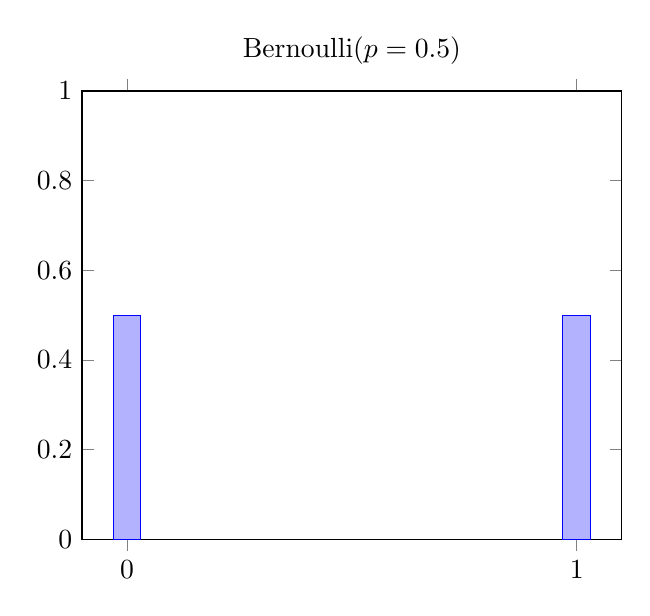
\begin{tikzpicture}
    \begin{axis}[ybar, symbolic x coords={0,1}, xtick=data, ymin=0, ymax=1, title={Bernoulli($p=0.5$)}]
        \addplot coordinates {(0,0.5) (1,0.5)};
    \end{axis}
\end{tikzpicture}

\section{Binomial Distribution}
The binomial distribution models the number of successes in $n$ independent Bernoulli trials:
\[ P(X = k) = \binom{n}{k} p^k (1 - p)^{n - k}, \quad k = 0,1,\dots,n. \]

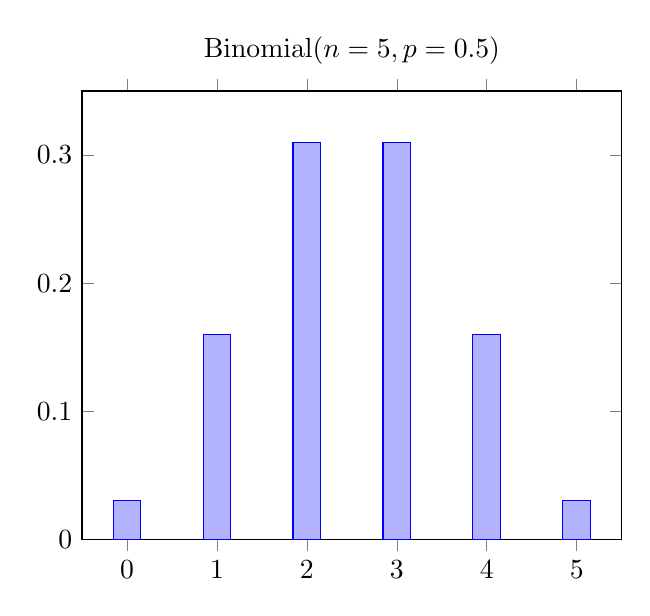
\begin{tikzpicture}
    \begin{axis}[ybar, symbolic x coords={0,1,2,3,4,5}, xtick=data, ymin=0, ymax=0.35, title={Binomial($n=5, p=0.5$)}]
        \addplot coordinates {(0,0.03) (1,0.16) (2,0.31) (3,0.31) (4,0.16) (5,0.03)};
    \end{axis}
\end{tikzpicture}

\section{Geometric Distribution}
Models the number of trials until the first success:
\[ P(X = k) = (1 - p)^{k - 1} p, \quad k = 1,2,3,\dots \]

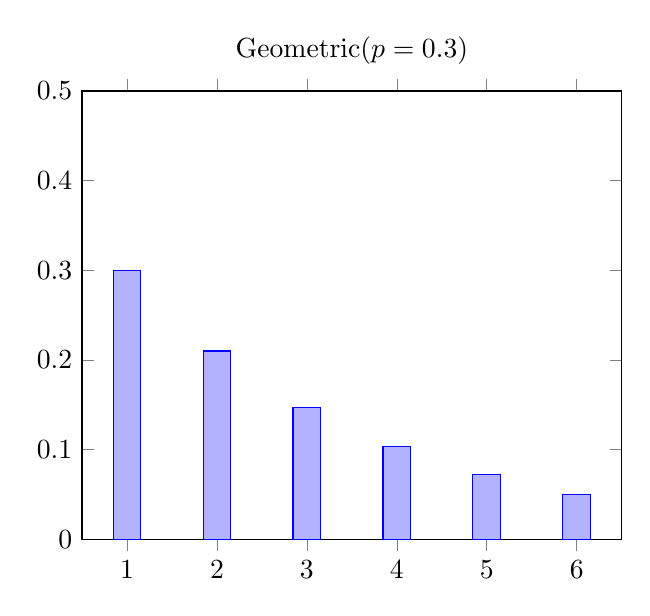
\begin{tikzpicture}
    \begin{axis}[ybar, symbolic x coords={1,2,3,4,5,6}, xtick=data, ymin=0, ymax=0.5, title={Geometric($p=0.3$)}]
        \addplot coordinates {(1,0.3) (2,0.21) (3,0.147) (4,0.103) (5,0.072) (6,0.05)};
    \end{axis}
\end{tikzpicture}

\section{Negative Binomial Distribution}
Models the number of trials needed to obtain $r$ successes:
\[ P(X = k) = \binom{k-1}{r-1} p^r (1 - p)^{k - r}, \quad k \geq r. \]

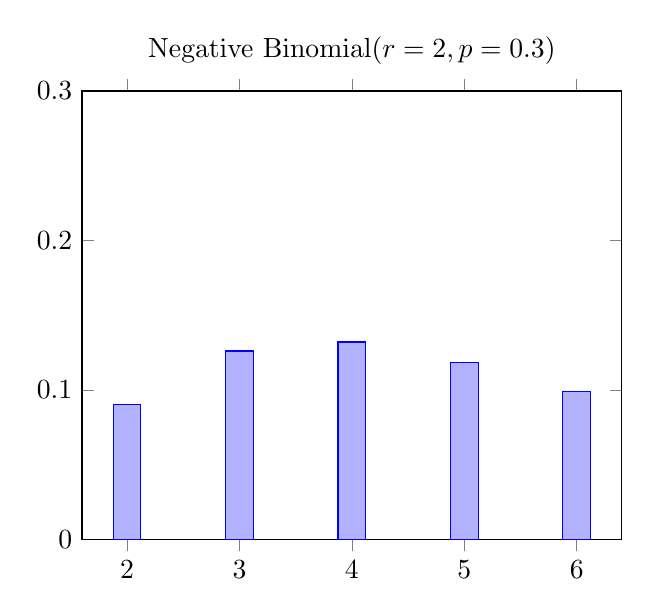
\begin{tikzpicture}
    \begin{axis}[ybar, symbolic x coords={2,3,4,5,6}, xtick=data, ymin=0, ymax=0.3, title={Negative Binomial($r=2, p=0.3$)}]
        \addplot coordinates {(2,0.09) (3,0.126) (4,0.132) (5,0.118) (6,0.099)};
    \end{axis}
\end{tikzpicture}

\section{Poisson Distribution}
Models the number of occurrences of an event in a fixed interval:
\[ P(X = k) = \frac{\lambda^k e^{-\lambda}}{k!}, \quad k = 0,1,2,\dots \]

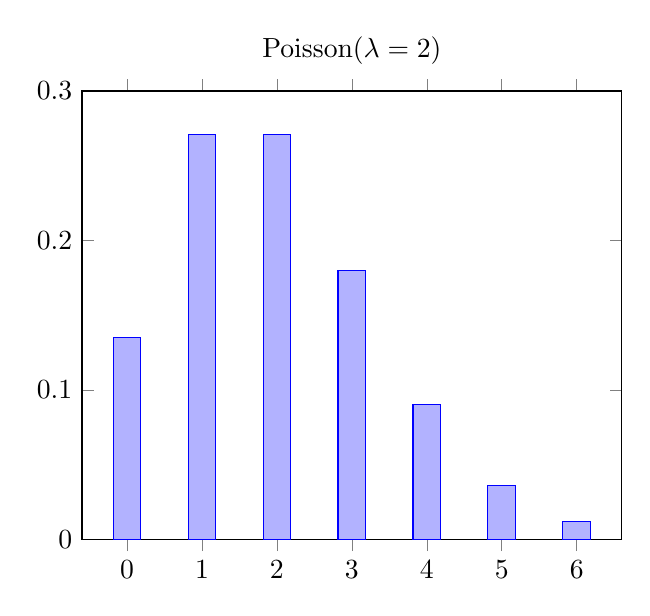
\begin{tikzpicture}
    \begin{axis}[ybar, symbolic x coords={0,1,2,3,4,5,6}, xtick=data, ymin=0, ymax=0.3, title={Poisson($\lambda=2$)}]
        \addplot coordinates {(0,0.135) (1,0.271) (2,0.271) (3,0.18) (4,0.09) (5,0.036) (6,0.012)};
    \end{axis}
\end{tikzpicture}

\section{Hypergeometric Distribution}
Models the number of successes in a sample drawn without replacement:
\[ P(X = k) = \frac{\binom{K}{k} \binom{N-K}{n-k}}{\binom{N}{n}}, \quad k = 0,1,2,\dots, \min(n, K). \]

\section{Discrete Uniform Distribution}
All values in a finite set are equally likely:
\[ P(X = k) = \frac{1}{n}, \quad k = 1,2,\dots,n. \]

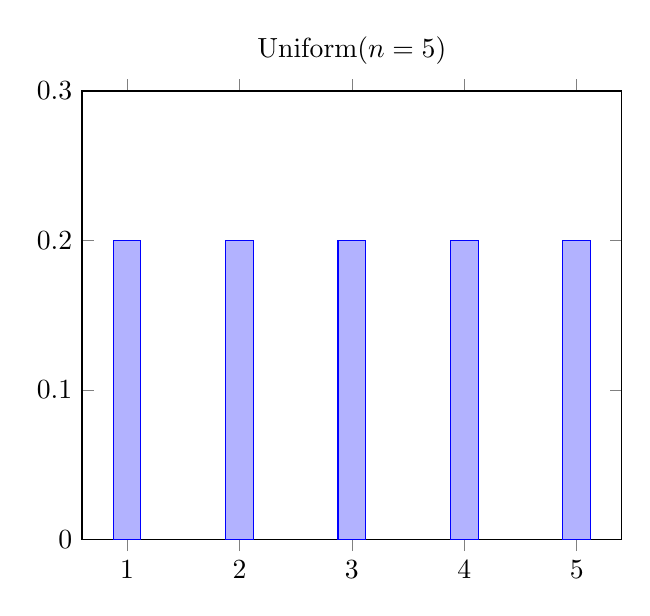
\begin{tikzpicture}
    \begin{axis}[ybar, symbolic x coords={1,2,3,4,5}, xtick=data, ymin=0, ymax=0.3, title={Uniform($n=5$)}]
        \addplot coordinates {(1,0.2) (2,0.2) (3,0.2) (4,0.2) (5,0.2)};
    \end{axis}
\end{tikzpicture}

\end{document}
